% \documentclass[10pt]{beamer} %slightly bigger font
\documentclass[aspectratio=169, 10pt]{beamer}
\usetheme{default} 
\setbeamertemplate{navigation symbols}{} %gets rid of navigation symbols
%\setbeamertemplate{footline}{} %gets rid of bottom navigation bars
%\setbeamertemplate{footline}[page number]{} %use this, if you want page numbers
%
\setbeamertemplate{itemize items}[circle] %I like round bullet points
%
\addtobeamertemplate{navigation symbols}{}{%
    \usebeamerfont{footline}%
    \usebeamercolor[fg]{title}%
    \hspace{5em}%
    \normalsize\insertframenumber/\inserttotalframenumber
}

\setlength\parskip{10pt} % I like white space between paragraphs

\setbeamertemplate{frametitle continuation}[from second][ ]

% Here is a `helper' functions to save typing, later
\newcommand{\mystart}[1]{ \section{#1}\begin{frame}[allowframebreaks, fragile] \frametitle{#1} } 

%\usepackage{float}
%\usepackage{bbm}
%\usepackage{amsmath}
%\usepackage{amssymb}
%\usepackage{ulem}
%\usepackage{subfig}
%\usepackage{sidecap}
%\usepackage{wrapfig}
%\usepackage{url}
%


\usepackage{graphicx}
\usepackage{wrapfig}
\usepackage{subfig}
\usepackage{sidecap}
\usepackage{fancyvrb}
\usepackage{algorithm}
\usepackage{algorithmic}

\newcommand{\xmark}{\ding{55}}%
\newcommand{\Ell}{\mathcal{L}}
\newcommand{\mb}{\mathbf}
\newcommand{\indfun}[1]{\ensuremath{\mb{1}_{\{#1\}}}}
\newcommand{\E}{\mathbbm{E}}
\DeclareMathOperator*{\argmin}{argmin}

\newcommand{\ind}{\mathbbm{1}}
\newcommand{\R}{\mathbb{R}}
\newcommand{\C}{\mathbb{C}}
\newcommand{\Z}{\mathbb{Z}}

\fvset{frame=none,framesep=0mm,fontsize=\tiny,numbers=none,framerule=0mm,numbersep=1mm,commandchars=\\\{\}}

%\mode<presentation>
%{
%  \usetheme{Boadilla}      % or try Darmstadt, Madrid, Warsaw, ...
%  \usecolortheme{beaver} % or try albatross, beaver, crane, ...
%  \usefonttheme{default}  % or try serif, structurebold, ...
%  \setbeamertemplate{navigation symbols}{}
%  \setbeamertemplate{caption}[numbered]
%
%
%}


%\usepackage{media9}
\usepackage{animate}

%% For \subfloat command
\usepackage{subfig}

\usepackage{color}
\newcommand{\blue}[1]{{\color{blue} #1} }
\newcommand{\red}[1]{{\color{red} #1} }
\definecolor{mygray}{rgb}{0.95,0.95,0.95}
\newcommand{\myGray}[1]{{\color{mygray} #1} }
\usepackage{tikz,pgfpages}
\usepackage{amsmath,amssymb}
\usetikzlibrary{shapes,arrows,trees,mindmap,decorations.pathreplacing}

\usepackage{algorithm,algorithmic}

\usepackage{cancel}

%\newcommand{\amp}{\mathop{\:\:\,}\nolimits}
%
%\newcommand{\prox}{\mathop{\rm prox}\nolimits}

\newtheorem{proposition}{Proposition}
%\newtheorem{example}{Example}
%\newtheorem{definition}{Definition}
\newcommand{\svskip}{\vspace{1.75mm}}
\def\E{\mathop{\rm E\,\!}\nolimits}
\def\Var{\mathop{\rm Var}\nolimits}
\def\Cov{\mathop{\rm Cov}\nolimits}
\def\trace{\mathop{\rm trace}\nolimits}
\def\logdet{\mathop{\rm \logdet}\nolimits}
\def\vec{\mathop{\rm vec}\nolimits}
\def\den{\mathop{\rm den}\nolimits}
\def\midd{\mathop{\,|\,}\nolimits}
\def\sgn{\mathop{\rm sgn}\nolimits}
\def\sinc{\mathop{\rm sinc}\nolimits}
\def\curl{\mathop{\rm curl}\nolimits}
\def\div{\mathop{\rm div}\nolimits}
\def\tr{\mathop{\rm tr}\nolimits}
\def\len{\mathop{\rm len}\nolimits}
\def\cond{\mathop{\rm cond}\nolimits}
\def\conv{\mathop{\rm conv}\nolimits}
\def\dom{\mathop{\rm dom}\nolimits}
\def\epi{\mathop{\rm epi}\nolimits}
\def\graph{\mathop{\rm graph}\nolimits}
\def\cl{\mathop{\rm cl}\nolimits}
\def\diag{\mathop{\rm diag}\nolimits}
\def\dist{\mathop{\rm dist}\nolimits}
\def\prox{\mathop{\rm prox}\nolimits}
\def\argmin{\mathop{\rm argmin}\nolimits}
\def\gph{\mathop{\rm gph}\nolimits}
\def\vec{\mathop{\rm vec}\nolimits}
\def\vech{\mathop{\rm vech}\nolimits}
\def\amp{\mathop{\;\:}\nolimits}
\newcommand{\ba}{\boldsymbol{a}}
\newcommand{\bb}{\boldsymbol{b}}
\newcommand{\bc}{\boldsymbol{c}}
\newcommand{\bd}{\boldsymbol{d}}
\newcommand{\be}{\boldsymbol{e}}
\newcommand{\bff}{\boldsymbol{f}}
\newcommand{\bg}{\boldsymbol{g}}
\newcommand{\bh}{\boldsymbol{h}}
\newcommand{\bi}{\boldsymbol{i}}
\newcommand{\bj}{\boldsymbol{j}}
\newcommand{\bk}{\boldsymbol{k}}
\newcommand{\bl}{\boldsymbol{l}}
\newcommand{\bm}{\boldsymbol{m}}
\newcommand{\bn}{\boldsymbol{n}}
\newcommand{\bo}{\boldsymbol{o}}
\newcommand{\bp}{\boldsymbol{p}}
\newcommand{\bq}{\boldsymbol{q}}
\newcommand{\br}{\boldsymbol{r}}
\newcommand{\bs}{\boldsymbol{s}}
\newcommand{\bt}{\boldsymbol{t}}
\newcommand{\bu}{\boldsymbol{u}}
\newcommand{\bv}{\boldsymbol{v}}
\newcommand{\bw}{\boldsymbol{w}}
\newcommand{\bx}{\boldsymbol{x}}
\newcommand{\by}{\boldsymbol{y}}
\newcommand{\bz}{\boldsymbol{z}}
\newcommand{\bA}{\boldsymbol{A}}
\newcommand{\bB}{\boldsymbol{B}}
\newcommand{\bC}{\boldsymbol{C}}
\newcommand{\bD}{\boldsymbol{D}}
\newcommand{\bE}{\boldsymbol{E}}
\newcommand{\bF}{\boldsymbol{F}}
\newcommand{\bG}{\boldsymbol{G}}
\newcommand{\bH}{\boldsymbol{H}}
\newcommand{\bI}{\boldsymbol{I}}
\newcommand{\bJ}{\boldsymbol{J}}
\newcommand{\bK}{\boldsymbol{K}}
\newcommand{\bL}{\boldsymbol{L}}
\newcommand{\bM}{\boldsymbol{M}}
\newcommand{\bN}{\boldsymbol{N}}
\newcommand{\bO}{\boldsymbol{O}}
\newcommand{\bP}{\boldsymbol{P}}
\newcommand{\bQ}{\boldsymbol{Q}}
\newcommand{\bR}{\boldsymbol{R}}
\newcommand{\bS}{\boldsymbol{S}}
\newcommand{\bT}{\boldsymbol{T}}
\newcommand{\bU}{\boldsymbol{U}}
\newcommand{\bV}{\boldsymbol{V}}
\newcommand{\bW}{\boldsymbol{W}}
\newcommand{\bX}{\boldsymbol{X}}
\newcommand{\bY}{\boldsymbol{Y}}
\newcommand{\bZ}{\boldsymbol{Z}}
\newcommand{\balpha}{\boldsymbol{\alpha}}
\newcommand{\bbeta}{\boldsymbol{\beta}}
\newcommand{\bgamma}{\boldsymbol{\gamma}}
\newcommand{\bdelta}{\boldsymbol{\delta}}
\newcommand{\bepsilon}{\boldsymbol{\epsilon}}
\newcommand{\blambda}{\boldsymbol{\lambda}}
\newcommand{\bmu}{\boldsymbol{\mu}}
\newcommand{\bnu}{\boldsymbol{\nu}}
\newcommand{\bphi}{\boldsymbol{\phi}}
\newcommand{\bpi}{\boldsymbol{\pi}}
\newcommand{\bsigma}{\boldsymbol{\sigma}}
\newcommand{\btheta}{\boldsymbol{\theta}}
\newcommand{\bzeta}{\boldsymbol{\zeta}}
\newcommand{\bomega}{\boldsymbol{\omega}}
\newcommand{\bGamma}{\boldsymbol{\Gamma}}
\newcommand{\bDelta}{\boldsymbol{\Delta}}
\newcommand{\bTheta}{\boldsymbol{\Theta}}
\newcommand{\bLambda}{\boldsymbol{\Lambda}}
\newcommand{\bXi}{\boldsymbol{\Xi}}
\newcommand{\bPi}{\boldsymbol{\Pi}}
\newcommand{\bSigma}{\boldsymbol{\Sigma}}
\newcommand{\bUpsilon}{\boldsymbol{\Upsilon}}
\newcommand{\bPhi}{\boldsymbol{\Phi}}
\newcommand{\bPsi}{\boldsymbol{\Psi}}
\newcommand{\bOmega}{\mathbf{\Omega}}

\newcommand{\source}[1]{\caption*{Source: {#1}} }
\newcommand{\indep}{\perp \!\!\! \perp}


% display footnote with no number
\newcommand\blfootnote[1]{%
\begingroup
\renewcommand\thefootnote{}\footnote{#1}%
\addtocounter{footnote}{-1}%
\endgroup
}





\title[]{False discovery rate control for polygenic risk prediction}
\author[Benjamin Chu]{Benjamin Chu}
% \institute[stanford]{
% 1/13/2022 group meeting
% }

% \date{4/14/2022 Sabatti group meeting}
\date{4/21/2022 CAPE meeting (online)}

%\epstopdfDeclareGraphicsRule{.gif}{png}{.png}{convert gif:#1 png:\OutputFile}
%\AppendGraphicsExtensions{.gif}

\AtBeginSection[]
{
 \begin{frame}<beamer>
 \frametitle{Outline}
 \tableofcontents[currentsection]
 \end{frame}
}
\includeonly{struct}

\setbeamercovered{transparent}
\begin{document}
\frame{\titlepage}


% \frame{
% \frametitle{Polygenic Risk Scores (PRS)}
% \begin{itemize}
%     \item PRS: build a model to predict \textit{complex} human traits using genetic (e.g. GWAS) data
%     \item We want our model to  \textbf{predict in different populations}, but most genetics data are from European samples 
% \end{itemize}
% \begin{figure}[ht]
%     \begin{minipage}[b]{0.45\linewidth}
%         \centering
%         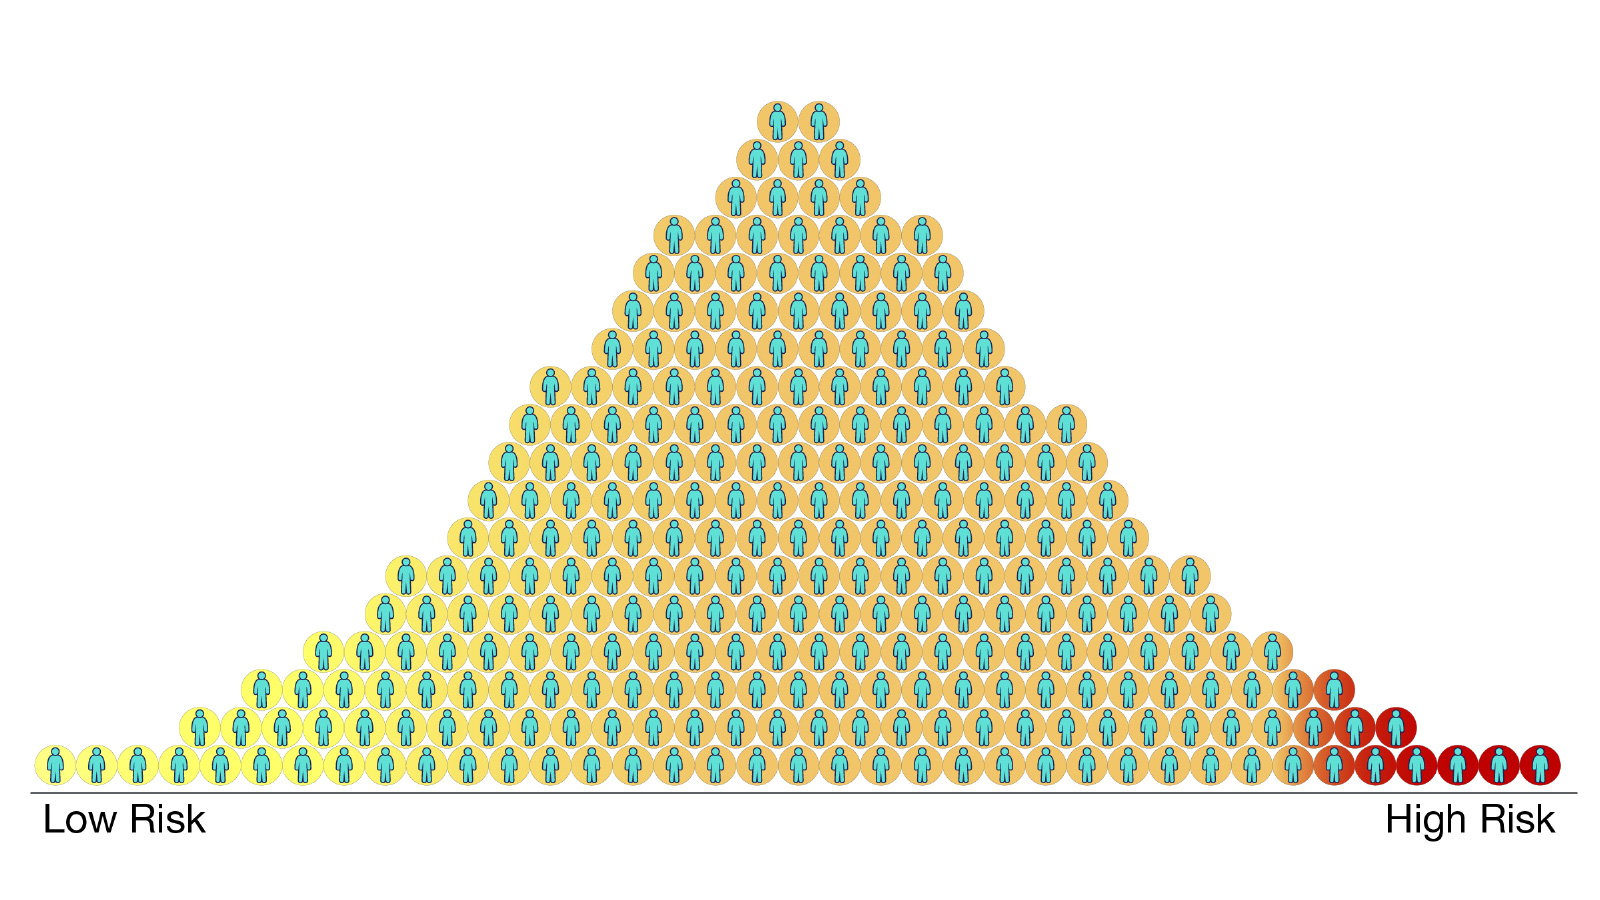
\includegraphics[width=\textwidth]{figures/prs-bell_0.jpg}
%         \vspace{0.5cm}
%         % \caption{Label for a}
%         % \label{fig:a}
%     \end{minipage}
%     \hspace{0.5cm}
%     \begin{minipage}[b]{0.45\linewidth}
%         \centering
%         \begin{table}[]
%             \centering
%             \begin{tabular}{c|c}
%                 Ancestry & \% samples \\
%                 \hline
%                 European & 78\%\\
%                 Asian & 10\%\\
%                 African & 2\%\\
%                 Hispanic & 1\%\\
%                 Other minorities & 0.5\%\\
%                 Unreported & 8.5\%\\
%             \end{tabular}
%             \caption{The percentage of ancestry populations included in large-scale genomic studies is overwhelmingly European}
%             \label{tab:my_label}
%         \end{table}
%         % 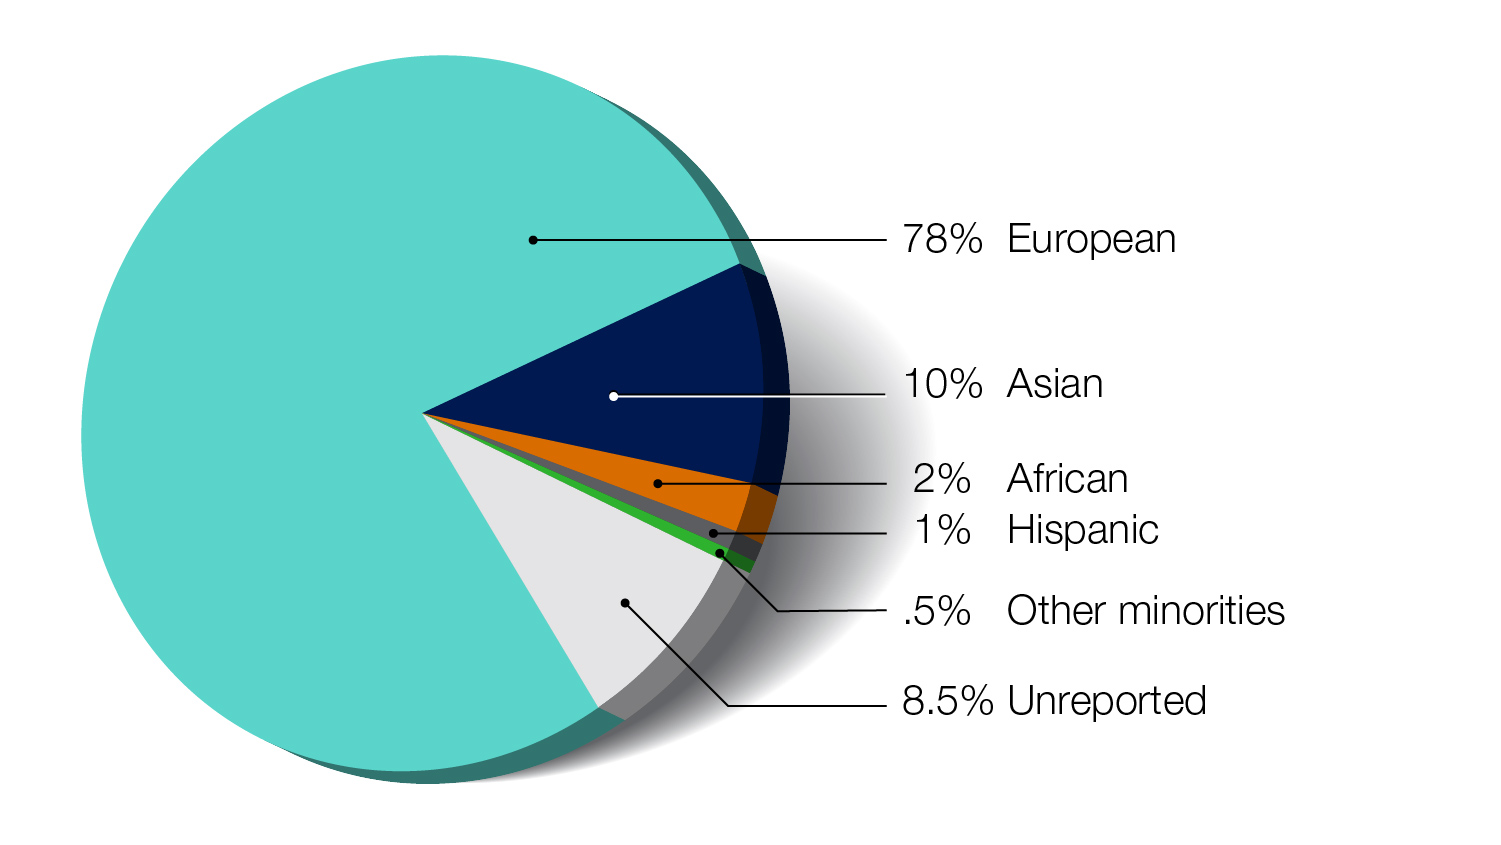
\includegraphics[width=1.2\textwidth]{figures/prs-diversity.jpg}
%         % \caption{Label for b}
%         % \label{fig:b}
%     \end{minipage}
% \end{figure}
% \blfootnote{Figure and data from: https://www.genome.gov/Health/Genomics-and-Medicine/Polygenic-risk-scores}
% }

\frame{
\frametitle{Methods for Polygenic Risk Scores (PRS)}
Goal of PRS: build a model to predict \textit{complex} human traits using genetic (e.g. GWAS) data.
\begin{itemize}
    \item \textbf{Clumping + thresholding} (C+T) \cite{choi2019prsice}
    \begin{enumerate}
        \item Remove highly correlated SNPs (before or after selection)
        \item Find significant SNPs passing \textit{loose p-value threshold}
        \item Estimate $\hat{\beta}_j$ from a univariate regression
        \item Predicted phenotype for sample $i$: $\hat{y}_i = \sum_{j} x_{ij}\hat{\beta}_j$
    \end{enumerate}
    \item \textbf{Penalized regression methods} e.g.
    \begin{align*}
        \hat{\bbeta} 
        &= \text{minimize } \ \|\by - \bX\bbeta\|^2 + \lambda \|\bbeta\|_1 & \text{(LASSO)}\\
        \hat{\bbeta} 
        &= \text{minimize } \ \|\by - \bX\bbeta\|^2 \text{ s.t. } \|\bbeta\|_0 \le k & \text{(IHT)}
    \end{align*}
    where $\lambda$ and $k$ are sparsity inducing parameters tuned by cross validation.
    \item Other alternatives: Bayesian methods (BayesR \cite{moser2015simultaneous}), T-Trees (random forest) ...etc
\end{itemize}
}


\frame{
\frametitle{Strength and (possible?) weakness of LASSO for PRS}
\begin{figure}[ht]
    \begin{minipage}[b]{0.45\linewidth}
        \centering
        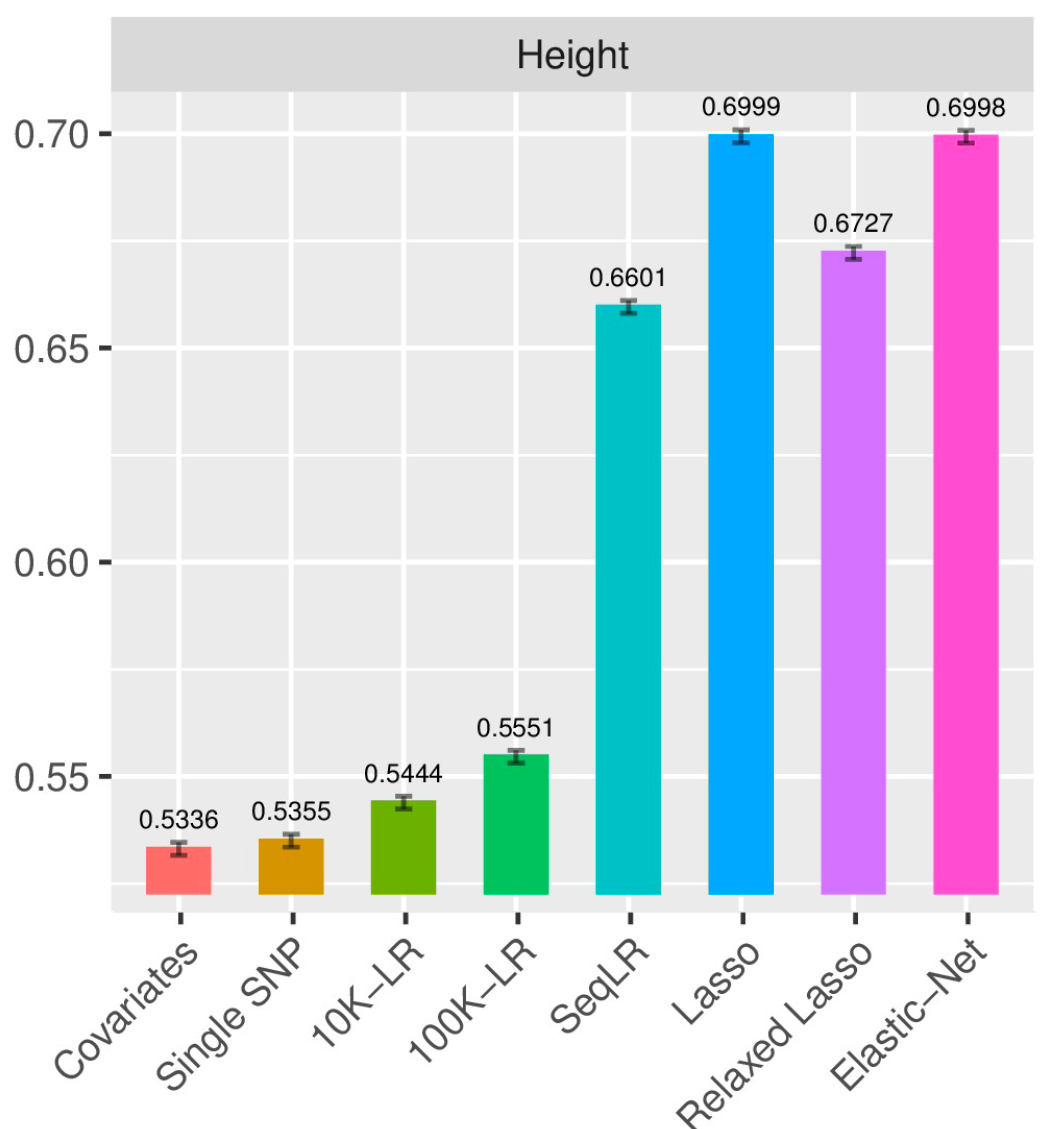
\includegraphics[width=0.95\textwidth]{figures/lasso-prs1.png}
    \end{minipage}
    \hspace{0.5cm}
    \begin{minipage}[b]{0.45\linewidth}
        \begin{itemize}
            \item LASSO/elastic-net typically outperforms other methods
            \item The number of non-zero beta for height is \alert{118,322}
            \item How does this model predict in other populations?
        \end{itemize}
        \vspace{2cm}
    \end{minipage}
\end{figure}
\blfootnote{Figure: Qian et al. 2020 (PLOS genetics), y-axis measures $R^2$ predictive performance}
}

\frame{
\frametitle{Problem: PRSs are population specific}
\begin{minipage}[b]{0.45\linewidth}
\begin{figure}
    \centering
    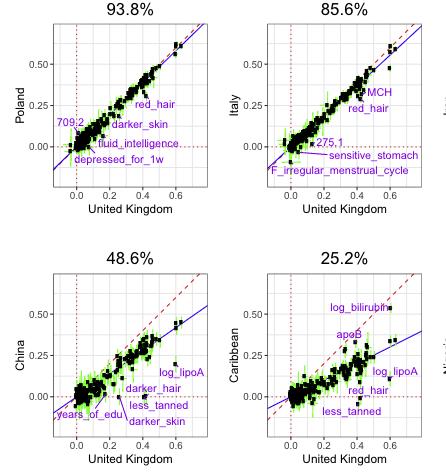
\includegraphics[width=0.8\textwidth]{figures/prive_AJHG_2022.png}
    \caption{Lasso study by Prive et al 2022 (AJHG). Prediction accuracy (partial $r^2$) drops across different group.}
\end{figure}
\end{minipage}
\hspace{0.7cm}
\begin{minipage}[b]{0.45\linewidth}
\begin{figure}
    \centering
    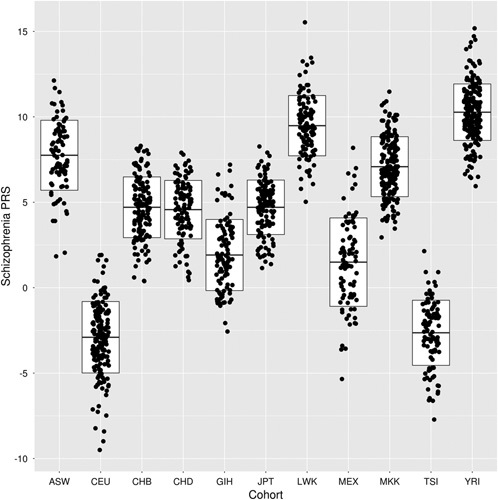
\includegraphics[width=0.8\textwidth]{figures/schizo_prs.jpeg}
    \caption{C+T study by David Curtis 2018 (Psychiatric Genetics). PRS for schizophrenia are highly sensitive to ethnic background}
\end{figure}
\end{minipage}

\centering
\alert{In both studies, a large number of predictors were selected. }
}

\frame{
\frametitle{PRS are population specific (but why?)}

Watch talks\footnote{https://cehg.stanford.edu/evolgenome-seminars} by Graham Coop and Jonathan Kaplan
\begin{itemize}
    \item Unmeasured (true) population differences
    \begin{itemize}
        \item Due to genetic drift/selection, which may not be surveyed
        \item Unmeasured environmental effects
    \end{itemize}
    \item Estimation bias
    \begin{itemize}
        \item Unadjusted confounders (e.g. population stratification) can produce excess false positive
        \item Imprecise effect size estimation (e.g. non-additive terms, interaction, epistasis...etc)
        \item Intrinsic problems with data (e.g. LD and rare alleles) that cannot be modeled well
    \end{itemize}
\end{itemize}
We will develop methods to address problems related to estimation bias. 
}

\begin{frame}{Idea for solution}
\begin{enumerate}
    \item Some papers\footnote{For example, \cite{abramovich2006adapting} and \cite{benjamini2009simple}} suggest controlling the number of \textbf{false discoveries} will help prediction
    \item Most PRS models include an enormous number of variants
    % \item Statistical knockoffs have recently been introduced for \textbf{variable selection}
    % \begin{itemize}
    %     \item Knockoffs work for covariates with arbitrary correlation structure, unlike e.g. Benjamini-Hochberg
    %     \item Knockoffs do not need valid p-values (thus we can quantify FDR of e.g. LASSO)
    % \end{itemize}
    \item \alert{Can prediction improve (broadly speaking) if we select a cleaner set of predictors?}
\end{enumerate}
Lets explore this idea with \textbf{Knockoffs}
\end{frame}

\begin{frame}{The Goals of Statistical Knockoffs}
Knockoffs are designed for two purpose:
\begin{itemize}
    \item Instead of controlling FWER\footnote{which is what Bonferroni correction does in GWAS}, the knockoff procedure controls the FDR
    \begin{align*}
        FDR = E\left(\frac{\# \text{false positives}}{\text{\# total discoveries}}\right)
    \end{align*}
    This significantly improves power.
    \item Knockoff based inference tests \textit{conditional hypotheses}. If $G$ is a SNP or a group of SNPs, we test
    \begin{align*}
        \mathcal{H}_0 = Y \indep X_G \ | \ X_{-G}
    \end{align*}
     Conditioning on $X_{-G}$ removes SNPs only marginally associated with the trait due to e.g. linkage disequilibrium, prioritizing causal associations
\end{itemize}
\end{frame}

\begin{frame}{Properties of Knockoffs}
\begin{itemize}
    \item The knockoff-filter wraps \textit{any} algorithm that provides \fbox{feature-importance scores} and helps us decide which variables to choose. 
    \begin{itemize}
        \item In particular, it does not need valid p-values (thus we can quantify FDR of e.g. LASSO)
        \item The selected variables have guaranteed FDR control. 
    \end{itemize}
    \item Knockoffs work for covariates with arbitrary correlation structure, unlike e.g. Benjamini-Hochberg
\end{itemize}
\end{frame}

\begin{frame}{The Knockoff procedure}
\begin{enumerate}
    \item For each sample $X \in \{0, 1, 2\}^p$, generate \textit{knockoffs} $\Tilde{X}\in\{0, 1, 2\}^{p}$ satisfying 
    \begin{itemize}
        \item $Y \indep \Tilde{X} \ | \ X$
        \item $(X, \Tilde{X}) \stackrel{d}{=} (X, \Tilde{X})_{\text{swap}(S)} \forall S$. E.g. If $S=\{2\}$, then $(X_1, X_2, X_3, \Tilde{X}_1, \Tilde{X}_2, \Tilde{X}_3) \stackrel{d}{=} (X_1, \alert{\tilde{X}_2}, X_3, \Tilde{X}_1, \alert{X_2}, \Tilde{X}_3)$
    \end{itemize}
    \item Compute feature importance statistic on concatenated matrix $\left[\bX \ \Tilde{\bX}\right]$
    \item Compute knockoff scores \fbox{$W_G = ImportanceScore(G)- ImportanceScore(\tilde{G})$} for all $G$s
    \item Choose all $G$ such that $W_G \ge \tau$, where $\tau$ depends on FDR threshold $q$ via 
    \begin{align*}
        \tau = \min \left\{t > 0 : \frac{1 + \#\{G: W_G \le -t\}}{\#\{j: W_G \ge t\} \vee 1} \le q\right\}
    \end{align*}
\end{enumerate}
\end{frame}

\begin{frame}{Knockoffs are successful for GWAS}
\begin{figure}
    \centering
    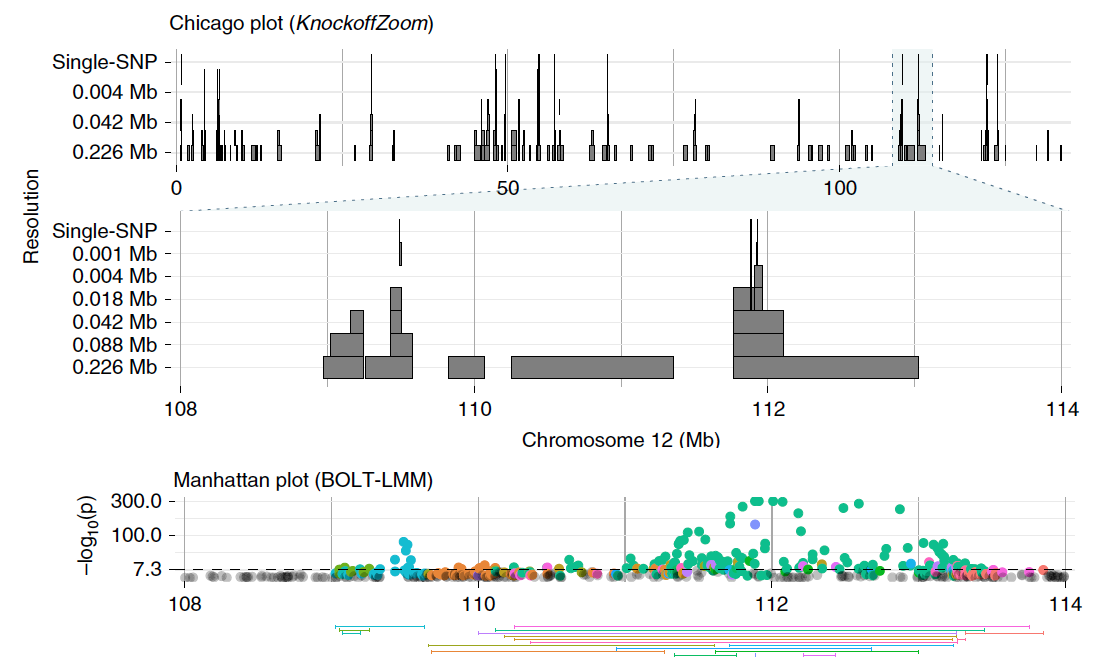
\includegraphics[width=0.65\textwidth]{figures/knockoffzoom.png}
\end{figure}
We previously found Knockoff-Lasso finds \textbf{more predictors} and \textbf{localizes} better than traditional LMM. 
\blfootnote{Figure: Sesia et al 2020 (Nature communications)}
\end{frame}

\begin{frame}{How to use Knockoffs for prediction?}
    Recall: We want to do prediction. 
    
    After Knockoffs select a set of $G$s, there are multiple ways to build a PRS model
    \begin{enumerate}
        \item If $G$s are singleton, we can use least squares to fit low-dimensional model on selected $G$s
        \item If $G$s are SNP groups, 
        \begin{itemize}
            \item Option 1: Run a second Lasso routine only allowing non-zero entries in selected $G$s
            \item Option 2: Run least squares fit on the non-zero entries of the selected $G$s
        \end{itemize}
    \end{enumerate}
\end{frame}

\begin{frame}{Method summary}
Goal: we want to build a PRS model that can predict across ethnically diverse populations.
\begin{enumerate}
    \item We start with PRS methods that have principled selection \textit{and} estimation procedures, such as LASSO and IHT penalized regression
    \item In practice, the best performing PRSs select absurdly many predictors (e.g. $>100$k for height), which raises \textit{portability} issues. 
    \item We will kill (hopefully false positives) predictors  by applying the knockoff filter, which will give us a \textbf{sparser set with guaranteed FDR control}
    \item \alert{This is an experimental project that uses Knockoffs in a new way. We do not have finalized results!}
\end{enumerate}
Does this procedure work?
\end{frame}

\begin{frame}{Experiment 1: Independent genotypes}
    \begin{itemize}
        \item Simulate $6000 \times 50000$ matrix $\bX$ by
        \begin{align*}
            x_{ij} \sim \text{Binomial}(2, p_j), \quad p_j \sim \text{Uniform}(0, 1)
        \end{align*}
        \item 5000 samples used as training data, 1000 samples for testing
        \item Pick $|\mathcal{S}_{\text{causal}}|=100$ causal SNPs chosen uniformly, $h^2 = 0.5$
        \item Simulate phenotypes (using standardized $\bX$):
        \begin{align*}
            y_i = \sum_{j \in \mathcal{S}_{\text{causal}}} x_{ij}\beta_j + \epsilon_i, \quad \beta_j \sim N\left(0, \sqrt{\frac{h^2}{2|\mathcal{S}_{\text{causal}}|}}\right), \quad \epsilon_i \sim N(0, 1-h^2).
        \end{align*}
    \end{itemize}
    Evaluate performance:
    \begin{align*}
        & R^2 = 1 - \frac{\|\by -\bX_{test}\hat{\bbeta}\|_2^2}{\|\by - \overline{\by}\|_2^2} \quad \text{(For predicting in same population)}\\
        & \text{Partial } r^2 \quad (\text{For predicting across populations})
    \end{align*}
\end{frame}

\begin{frame}{Experiment 1 results: Independent genotypes}
    \begin{table}
        \begin{tabular}{ c|c|c|c|c } 
            \hline
            & LASSO & LASSO-ko & IHT & IHT-ko \\
            \hline
            $R^2$ & 0.42 & 0.46 & 0.45 & 0.45 \\
            power & 0.68 & 0.56 & 0.55 & 0.53\\
            FDR & 0.83 & 0.11 & 0.08 & 0.04 \\
            \hline
        \end{tabular}
        \caption{Single SNP knockoff results with target FDR = 0.1, averaged over 100 runs}
    \end{table}
    \begin{itemize}
        \item $R^2$ performance: LASSO-ko $\ge$ IHT-ko $=$ IHT $>$ LASSO
        \item Knockoffs control FDR, pay a small price in power
    \end{itemize}
\end{frame}

\begin{frame}{Experiment 2: UK Biobank genotypes}
    UK Biobank: $\sim$ 500,000 samples, primarily British but includes numerous other ethnicities. After QC, we retain
    \begin{table}[]
    \centering
    \small
    \begin{tabular}{c|c|c}
        Population & Sample size & Description\\
        \hline
        British & 320094 & \\
        Irish & 1066 & \\
        White & 15348 & \\
        Pakistani & 1617 & \\
        Bangladeshi & 213 & \\
        Indian  & 5188 & \\
        White and Asian & 722 & Mixed \\
        Chinese & 1442 & \\
        Asian & 1695 & \\
        Caribbean  & 3859 & \\
        White and Black & 912 & Mixed\\
        African  & 3112 & \\
    \end{tabular}
\end{table}
\end{frame}

\begin{frame}{Experiment 2 setup}
    \begin{itemize}
        \item Train data: chromosome 10 (29,481 SNPs) of UK Biobank with 10,000 British samples (i.e. very small subset)
        \item Phenotypes: $\by$ simulated in the same way as before, i.e. 
        \begin{itemize}
            \item Pick $|\mathcal{S}_{\text{causal}}|=100, 1000$ causal SNPs chosen uniformly, $h^2 = 0.5$
        \item Simulate phenotypes (using standardized $\bX$):
        \begin{align*}
            y_i = \sum_{j \in \mathcal{S}_{\text{causal}}} x_{ij}\beta_j + \epsilon_i, \quad \beta_j \sim N\left(0, \sqrt{\frac{h^2}{2|\mathcal{S}_{\text{causal}}|}}\right), \quad \epsilon_i \sim N(0, 1-h^2).
        \end{align*}
        \end{itemize}
        \item Test data: all samples in UKB stratified by ethnicity
    \end{itemize}
\end{frame}

\begin{frame}{UKB experiments Lasso results (100/29481 SNPs causal, n=10000)}
    \begin{minipage}[b]{0.65\linewidth}
        \begin{figure}
            \centering
            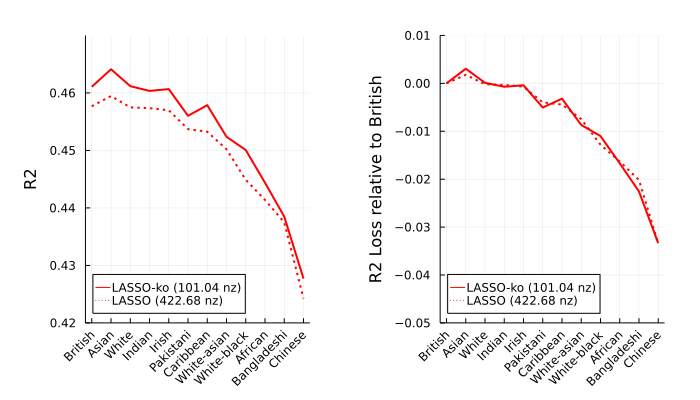
\includegraphics[width=\textwidth]{figures/k100_n10000_lasso.png}
            \begin{table}[]
                \centering
                \small
                \begin{tabular}{c|c|c}
                & LASSO & LASSO-ko\\
                \hline
                 \# nonzero $\hat{\beta}$ & 422.7 & 458.9\\
                 \# $\hat{\beta}$ selected & 422.7 & 101.0\\
                 power (group power) & 0.76 & 0.66 (0.70)\\
                 FDR (group FDR) & 0.82 & 0.34 (0.12)\\
                 \hline
            \end{tabular}
            \caption{Group knockoff (res5) results with target FDR = 0.1}
    \end{table}
    \end{figure}
    \end{minipage}
    \hspace{0.5cm}
    \begin{minipage}[b]{0.25\linewidth}
        \begin{itemize}
            \item Lasso have \textit{better power} but finds a lot of junk
            \item \alert{Knockoffs improves FDR in exchange for power}. 
            \item Here, the trade-off improved prediction.
        \end{itemize}
        \vspace{3cm}
    \end{minipage}
\end{frame}

\begin{frame}{UKB experiments results (100/29481 SNPs causal, n=10000)}
    \begin{minipage}[b]{0.65\linewidth}
        \begin{figure}
            \centering
            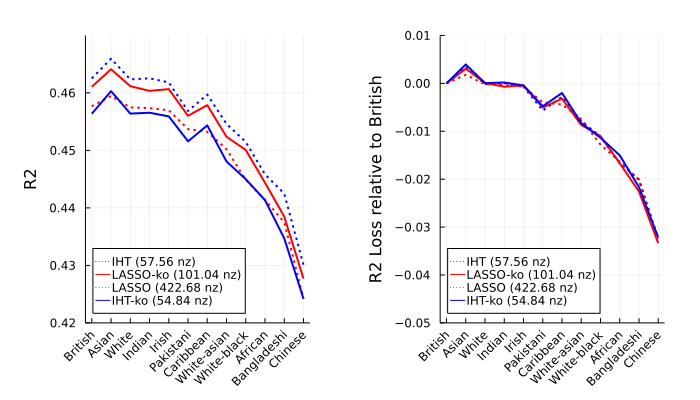
\includegraphics[width=\textwidth]{figures/k100_n10000.png}
            \begin{table}[]
                \centering
                \small
                \begin{tabular}{c|c|c|c|c}
                & IHT & IHT-ko & LASSO & LASSO-ko\\
                \hline
                 \# nonzero $\hat{\beta}$ & 57.6 & 56.6 & 422.7 & 458.9\\
                 \# $\hat{\beta}$ selected & 57.6 & 54.84 & 422.7 & 101.0\\
                 power (group power) & 0.54 & 0.52 (0.57) & 0.76 & 0.66 (0.70)\\
                 FDR (group FDR) & 0.05 & 0.04 (0.01) & 0.82 & 0.34 (0.12)\\
                 \hline
            \end{tabular}
            \caption{Group knockoff (res5) results with target FDR = 0.1}
    \end{table}
    \end{figure}
    
    \end{minipage}
    \hspace{0.5cm}
    \begin{minipage}[b]{0.25\linewidth}
        \begin{itemize}
            \item Standard IHT has good power and controlled FDR
            \item If FDR was good to start out with, knockoffs hurt prediction performance
        \end{itemize}
        \vspace{3cm}
    \end{minipage}
\end{frame}


\begin{frame}{UKB experiments results (500/29481 SNPs causal, n=10000)}
    \begin{minipage}[b]{0.65\linewidth}
        \begin{figure}
            \centering
            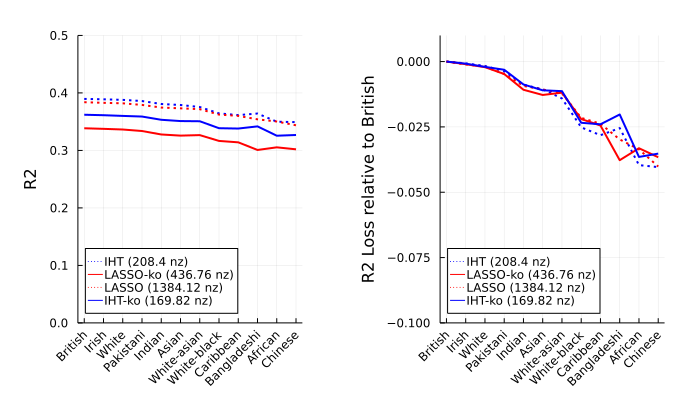
\includegraphics[width=0.9\textwidth]{figures/k500_n10000.png}
            \begin{table}[]
                \centering
                \small
                \begin{tabular}{c|c|c|c|c}
                & IHT & IHT-ko & LASSO & LASSO-ko\\
                \hline
                 \# nonzero $\hat{\beta}$ & 208.4 & 190.42 & 1384.12 & 1537.5\\
                 \# $\hat{\beta}$ selected & 208.4 & 169.82 & 1384.12 & 436.76\\
                 power  (group power) & 0.36 & 0.30 (0.44) & 0.55 & 0.39 (0.57)\\
                 FDR  (group FDR) & 0.17 & 0.12 (0.02) & 0.80 & 0.55 (0.17)\\
                 \hline
            \end{tabular}
            \caption{Group knockoff (res5) results with target FDR = 0.25}
    \end{table}
    \end{figure}
    
    \end{minipage}
    \hspace{0.5cm}
    \begin{minipage}[b]{0.25\linewidth}
        % \begin{itemize}
        %     \item some text
        % \end{itemize}
        % \vspace{3cm}
    \end{minipage}
\end{frame}


\begin{frame}{UKB experiments results (1000/29481 SNPs causal, n=10000)}
    \begin{minipage}[b]{0.65\linewidth}
        \begin{figure}
            \centering
            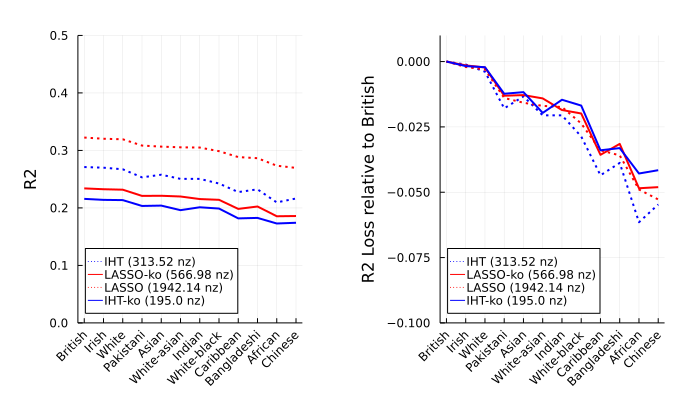
\includegraphics[width=0.9\textwidth]{figures/k1000_n10000.png}
            \begin{table}[]
                \centering
                \small
                \begin{tabular}{c|c|c|c|c}
                & IHT & IHT-ko & LASSO & LASSO-ko\\
                \hline
                 \# nonzero $\hat{\beta}$ & 313.5 & 489.1 & 1942.1 & 2053.4\\
                 \# $\hat{\beta}$ selected & 313.5 & 195.0 & 1942.14 & 567.0\\
                 power (group power) & 0.21 & 0.14 (0.30) & 0.43 & 0.25 (0.48)\\
                 FDR (group FDR) & 0.28 & 0.25 (0.03) & 0.78 & 0.57 (0.098)\\
                 \hline
            \end{tabular}
            \caption{Group knockoff (res5) results with target group FDR 0.25}
    \end{table}
    \end{figure}
    
    \end{minipage}
    \hspace{0.5cm}
    \begin{minipage}[b]{0.25\linewidth}
        \begin{itemize}
            \item \alert{Knockoffs traded too much power for FDR improvements}
            \item Knockoffs predicts worse overall, but its performance degrade less
        \end{itemize}
        \vspace{3cm}
    \end{minipage}
\end{frame}

\begin{frame}{UKB experiments results (1000/29481 causal SNPs, n=20k)}
    \begin{minipage}[b]{0.65\linewidth}
        \begin{figure}
            \centering
            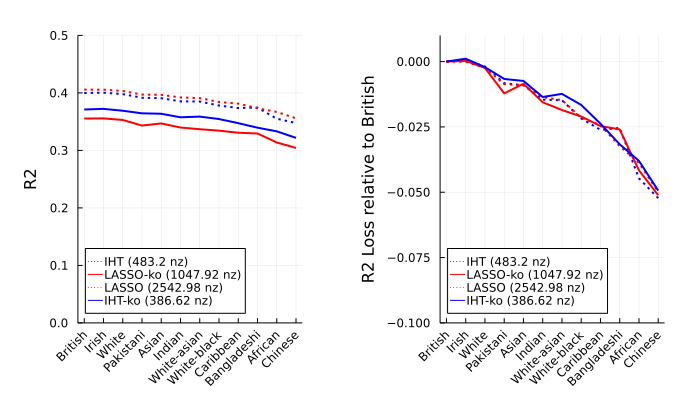
\includegraphics[width=0.9\textwidth]{figures/k1000_n20000.png}
            \begin{table}[]
                \centering
                \small
                \begin{tabular}{c|c|c|c|c}
                & IHT & IHT-ko & LASSO & LASSO-ko\\
                \hline
                 \# nonzero $\hat{\beta}$ & 483.2 & 482.72 & 2542.98 & 2796.3\\
                 \# $\hat{\beta}$ selected & 483.2 & 386.62 & 2542.98 & 1047.92\\
                 power (group power) & 0.37 & 0.32 (0.56) & 0.59 & 0.44 (0.72)\\
                 FDR (group FDR) & 0.21 & 0.17 (0.02) & 0.77 & 0.58 (0.12)\\
                 \hline
            \end{tabular}
            \caption{Group knockoff (res5) results with target FDR = 0.25}
    \end{table}
    \end{figure}
    
    \end{minipage}
    \hspace{0.5cm}
    \begin{minipage}[b]{0.25\linewidth}
        % \begin{itemize}
        %     \item 
        % \end{itemize}
        \vspace{3cm}
    \end{minipage}
\end{frame}

\begin{frame}{UKB experiments results (1000/29481 causal SNPs, n=50k)}
    \begin{minipage}[b]{0.65\linewidth}
        \begin{figure}
            \centering
            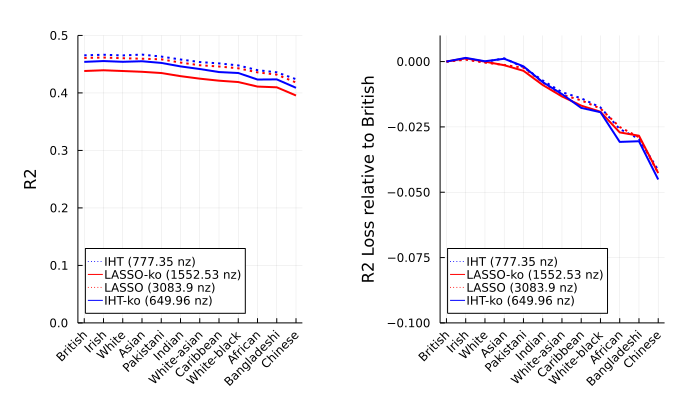
\includegraphics[width=0.9\textwidth]{figures/k1000_n50000.png}
            \begin{table}[]
                \centering
                \small
                \begin{tabular}{c|c|c|c|c}
                & IHT & IHT-ko & LASSO & LASSO-ko\\
                \hline
                 \# nonzero $\hat{\beta}$ & 777.347 & 797.122 & 3083.9 & 3429.8\\
                 \# $\hat{\beta}$ selected & 777.347 & 649.959 & 3083.9 & 1552.53\\
                 power (group power) & 0.58 & 0.53 (0.76) & 0.73 & 0.63 (0.87)\\
                 FDR (group FDR) & 0.22 & 0.16 (0.03) & 0.76 & 0.59 (0.15)\\
                 \hline
            \end{tabular}
            \caption{Group knockoff (res5) results with target FDR = 0.25}
    \end{table}
    \end{figure}
    
    \end{minipage}
    \hspace{0.5cm}
    \begin{minipage}[b]{0.25\linewidth}
        % \begin{itemize}
        %     \item 
        % \end{itemize}
        \vspace{3cm}
    \end{minipage}
\end{frame}

% \begin{frame}{Simulation summary}
%     When there are few SNPs with large effects
%     \begin{itemize}
%         \item LASSO admits a lot of false discoveries
%         \item Controlling FDR improves prediction performance
%     \end{itemize}
%     When trait is highly polymorphic, each with small effect
%     \begin{itemize}
%         \item Sparser models (knockoffs or IHT) kill too many predictors
%         \item Knockoffs predict worse overall but its performance degrade less
%     \end{itemize}
% \end{frame}

\begin{frame}{Full UK Biobank analysis}
\begin{itemize}
    \item Fit model on 80\% British samples (256,075 samples and 591,513 SNPs)
    \item Test on 20\% British samples (64,019 samples) and all other ethnicities
    \item Nongenetic covariates: sex, age, PC1-5
    \item Phenotypes: Height and systopic blood pressure (both continuous)
\end{itemize}
\end{frame}

\begin{frame}{UKB analysis: Height}
    \begin{figure}
        \centering
        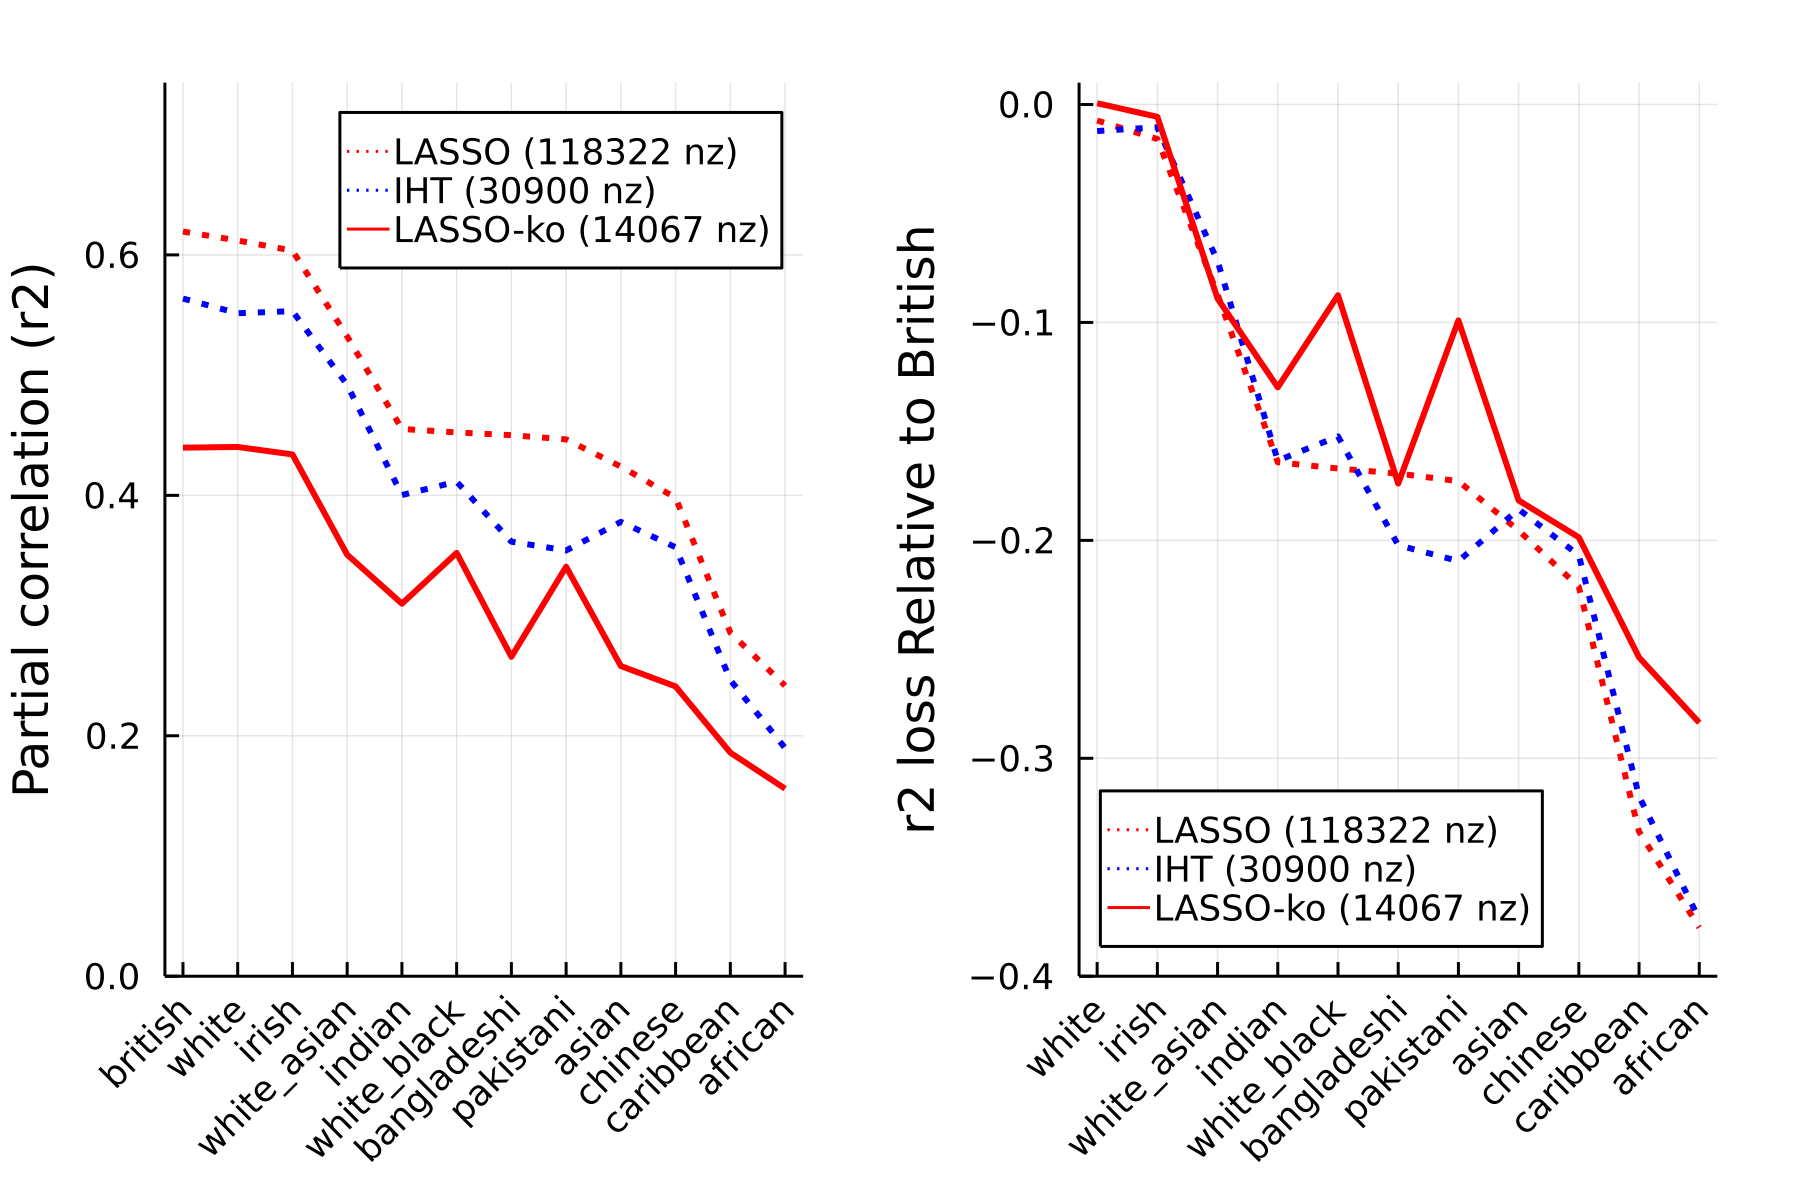
\includegraphics[width=0.7\textwidth]{figures/ukb_height.png}
    \end{figure}
    For highly polygenic trait, a more polygenic model is needed for better prediction, but knockoff model is more portable across population
\end{frame}

% \begin{frame}{UKB analysis: Platelet}
%     \begin{figure}
%         \centering
%         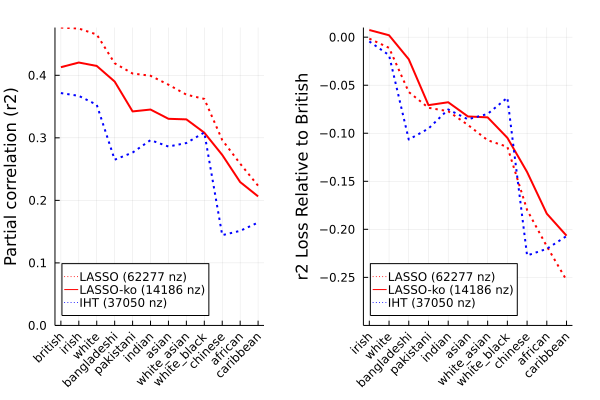
\includegraphics[width=0.6\textwidth]{figures/ukb_platelet.png}
%     \end{figure}
% \end{frame}

\begin{frame}{UKB analysis: Systolic Blood Pressure}
    \begin{figure}
        \centering
        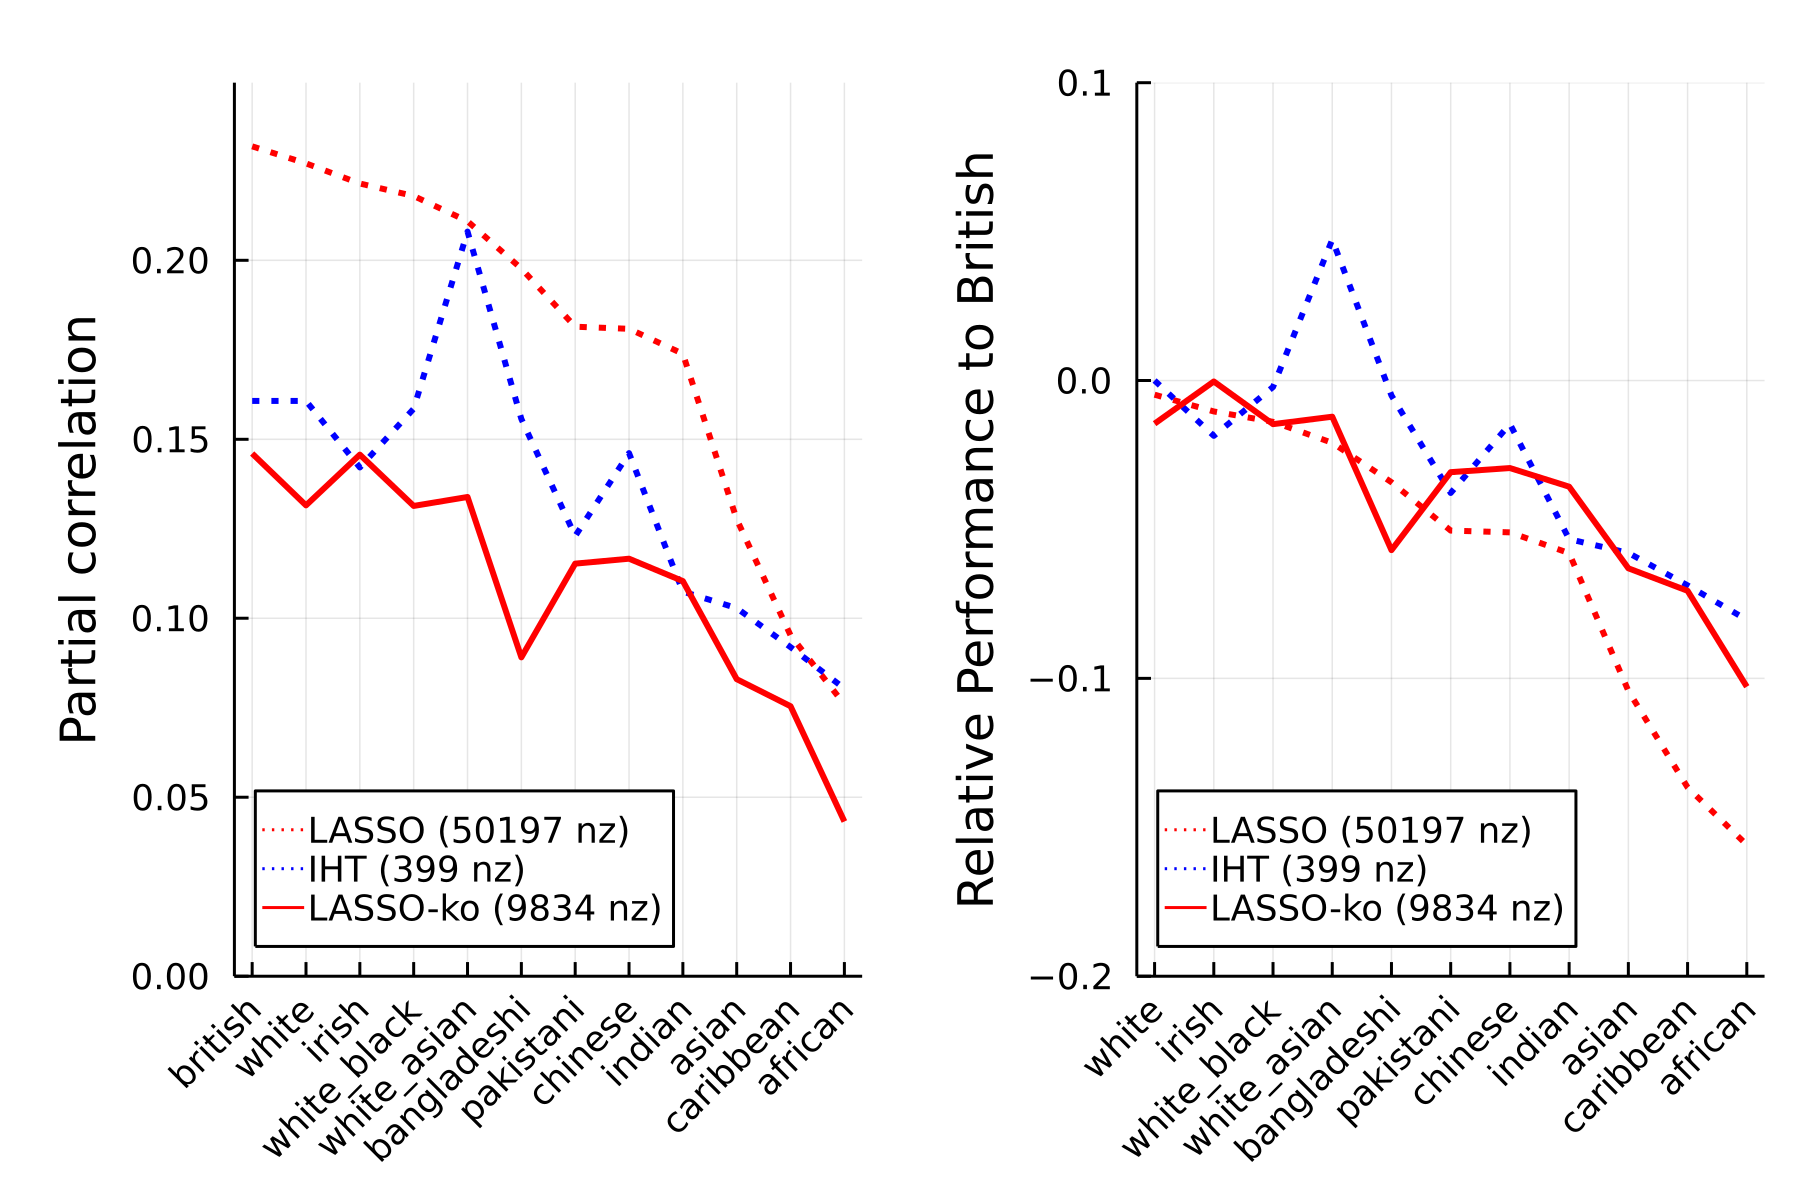
\includegraphics[width=0.6\textwidth]{figures/ukb_sbp.png}
    \end{figure}
    For highly polygenic trait, a more polygenic model is needed for better prediction, but sparser model is more portable across population
\end{frame}

\begin{frame}{Summary}
We are exploring a novel application of the knockoff framework for PRS prediction
\begin{itemize}
    \item The knockoff filter gives us a way to control FDR to a desired level, \textbf{in exchange for power} 
    \item This trade-off tends to be more "worth it" when the number of causal variants is low
    \item Knockoff filter may give worse prediction, but \textbf{it suffers less performance degradation} across populations
    \item We do not have real data example where knockoff models predict better in absolute scale, but we have only looked at very polygenic traits 
\end{itemize}
\end{frame}

\begin{frame}{Interested in Knockoffs?}
Main theory papers:
\begin{itemize}
    \item Barber, Rina Foygel, and Emmanuel J. Candès. "Controlling the false discovery rate via knockoffs." The Annals of Statistics 43, no. 5 (2015): 2055-2085.
    \item Candes, Emmanuel, Yingying Fan, Lucas Janson, and Jinchi Lv. "Panning for gold:‘model‐X’knockoffs for high dimensional controlled variable selection." Journal of the Royal Statistical Society: Series B (Statistical Methodology) 80, no. 3 (2018): 551-577.
\end{itemize}
Genetics application papers:
\begin{itemize}
    \item Sesia, Matteo, Eugene Katsevich, Stephen Bates, Emmanuel Candès, and Chiara Sabatti. "Multi-resolution localization of causal variants across the genome." Nature communications 11, no. 1 (2020): 1-10.
    \item Sesia, Matteo, Stephen Bates, Emmanuel Candès, Jonathan Marchini, and Chiara Sabatti. "False discovery rate control in genome-wide association studies with population structure." Proceedings of the National Academy of Sciences 118, no. 40 (2021).
\end{itemize}
\end{frame}

% \begin{frame}{Group knockoffs in tables}
%     \begin{figure}
%         \centering
%         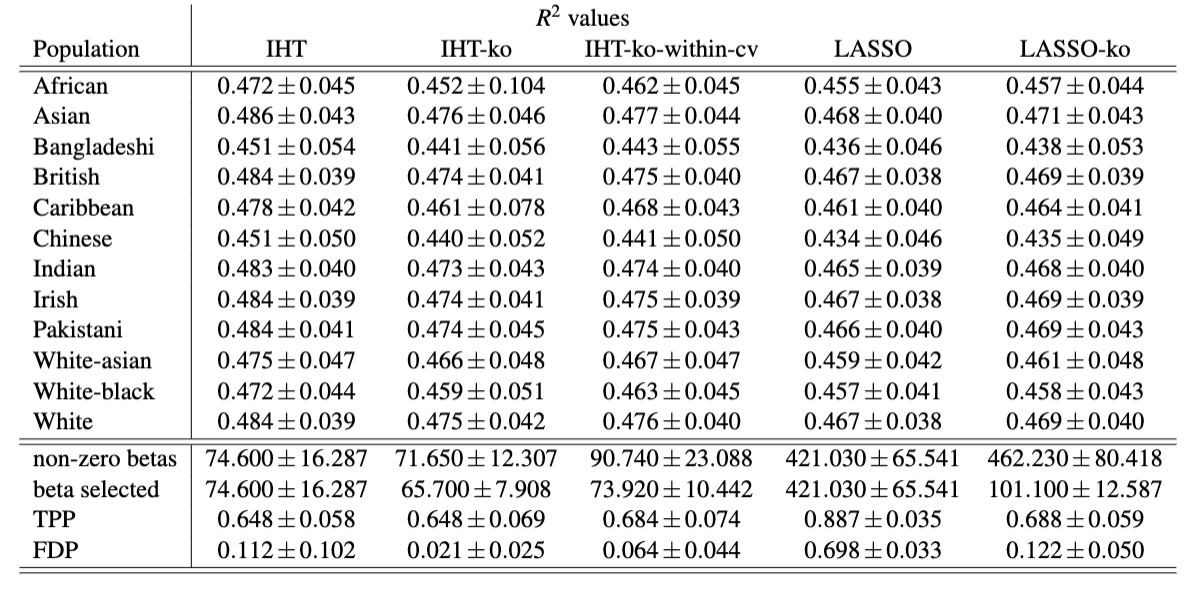
\includegraphics[width=\textwidth]{figures/Radj5_fdr0.1.png}
%     \end{figure}
%     LASSO group knockoffs have similar prediction to lasso no-knockoffs, while controlling  FDR. IHT-group knockoff predicts slightly worse.
% \end{frame}

References
\footnotesize
\bibliographystyle{apalike}
\bibliography{references}


\end{document}
